% Created 2025-05-21 Wed 07:42
% Intended LaTeX compiler: pdflatex
\documentclass[a4paper,12pt]{article}
\usepackage[utf8]{inputenc}
\usepackage[T1]{fontenc}
\usepackage{amsmath}
\usepackage{amssymb}
\usepackage{capt-of}
\usepackage{hyperref}
\usepackage{amsthm}
\usepackage{amssymb}
\usepackage{mathtools}
%\documentclass[12pt]{article}
\usepackage{geometry}

\usepackage{amsmath}
\usepackage{amssymb,amsfonts,textcomp}
\usepackage[T1]{fontenc}
\usepackage[utf8]{inputenc}
\usepackage{times} % Times New Roman font
\usepackage{setspace}
\usepackage[pdftex]{graphicx}

\usepackage{hyperref}

% Set line spacing to 1.5
\setstretch{1.5}

\geometry{a4paper, portrait, margin=0.7in, nohead}

\usepackage{titlesec}
\titleformat{\section}[block]{\normalfont\large\bfseries}{\thesection}{1em}{}
\titleformat{\subsection}[block]{\normalfont\large\bfseries}{\thesubsection}{1em}{}

\makeatletter

\newcommand{\student}[1]{\author{#1}}

\newcommand{\group}[1]{\def\@group{#1}}

\newcommand{\prof}[1]{\def\@prof{#1}}
\newcommand{\profdep}[1]{\def\@profdep{#1}}

\newcommand{\labno}[1]{\def\@labno{#1}}

\newcommand{\labtopic}[1]{\title{#1}}

\group{FAF--233}
\prof{Fistic Cristofor}
\profdep{sea, fcim utm}
\labno{4}

%% ox-latex features:
%   !announce-start, !guess-pollyglossia, !guess-babel, !guess-inputenc,
%   engraved-code, caption, maths, image, !announce-end.

% Setup for code blocks [1/2]

\usepackage{fvextra}

\fvset{%
  commandchars=\\\{\},
  highlightcolor=white!95!black!80!blue,
  breaklines=true,
  breaksymbol=\color{white!60!black}\tiny\ensuremath{\hookrightarrow}}

% Make line numbers smaller and grey.
\renewcommand\theFancyVerbLine{\footnotesize\color{black!40!white}\arabic{FancyVerbLine}}

\usepackage{xcolor}

% In case engrave-faces-latex-gen-preamble has not been run.
\providecolor{EfD}{HTML}{f7f7f7}
\providecolor{EFD}{HTML}{28292e}

% Define a Code environment to prettily wrap the fontified code.
\usepackage[breakable,xparse]{tcolorbox}
\providecommand{\codefont}{\footnotesize}
\DeclareTColorBox[]{Code}{o}%
{colback=EfD!98!EFD, colframe=EfD!95!EFD,
  fontupper=\setlength{\fboxsep}{0pt}\codefont,
  colupper=EFD,
  IfNoValueTF={#1}%
  {boxsep=2pt, arc=2.5pt, outer arc=2.5pt,
    boxrule=0.5pt, left=2pt}%
  {boxsep=2.5pt, arc=0pt, outer arc=0pt,
    boxrule=0pt, leftrule=1.5pt, left=0.5pt},
  right=2pt, top=1pt, bottom=0.5pt,
  breakable}

% Support listings with captions
\usepackage{float}
\floatstyle{plain}
\newfloat{listing}{htbp}{lst}
\newcommand{\listingsname}{Listing}
\floatname{listing}{\listingsname}
\newcommand{\listoflistingsname}{List of Listings}
\providecommand{\listoflistings}{\listof{listing}{\listoflistingsname}}


% Setup for code blocks [2/2]: syntax highlighting colors

\newcommand\efstrut{\vrule height 2.1ex depth 0.8ex width 0pt}
\definecolor{EFD}{HTML}{000000}
\definecolor{EfD}{HTML}{ffffff}
\newcommand{\EFD}[1]{\textcolor{EFD}{#1}} % default
\definecolor{EFh}{HTML}{7f7f7f}
\newcommand{\EFh}[1]{\textcolor{EFh}{#1}} % shadow
\definecolor{EFsc}{HTML}{228b22}
\newcommand{\EFsc}[1]{\textcolor{EFsc}{\textbf{#1}}} % success
\definecolor{EFw}{HTML}{ff8e00}
\newcommand{\EFw}[1]{\textcolor{EFw}{\textbf{#1}}} % warning
\definecolor{EFe}{HTML}{ff0000}
\newcommand{\EFe}[1]{\textcolor{EFe}{\textbf{#1}}} % error
\definecolor{EFc}{HTML}{b22222}
\newcommand{\EFc}[1]{\textcolor{EFc}{#1}} % font-lock-comment-face
\definecolor{EFcd}{HTML}{b22222}
\newcommand{\EFcd}[1]{\textcolor{EFcd}{#1}} % font-lock-comment-delimiter-face
\definecolor{EFs}{HTML}{8b2252}
\newcommand{\EFs}[1]{\textcolor{EFs}{#1}} % font-lock-string-face
\definecolor{EFd}{HTML}{8b2252}
\newcommand{\EFd}[1]{\textcolor{EFd}{#1}} % font-lock-doc-face
\definecolor{EFm}{HTML}{008b8b}
\newcommand{\EFm}[1]{\textcolor{EFm}{#1}} % font-lock-doc-markup-face
\definecolor{EFk}{HTML}{9370db}
\newcommand{\EFk}[1]{\textcolor{EFk}{#1}} % font-lock-keyword-face
\definecolor{EFb}{HTML}{483d8b}
\newcommand{\EFb}[1]{\textcolor{EFb}{#1}} % font-lock-builtin-face
\definecolor{EFf}{HTML}{0000ff}
\newcommand{\EFf}[1]{\textcolor{EFf}{#1}} % font-lock-function-name-face
\definecolor{EFv}{HTML}{a0522d}
\newcommand{\EFv}[1]{\textcolor{EFv}{#1}} % font-lock-variable-name-face
\definecolor{EFt}{HTML}{228b22}
\newcommand{\EFt}[1]{\textcolor{EFt}{#1}} % font-lock-type-face
\definecolor{EFo}{HTML}{008b8b}
\newcommand{\EFo}[1]{\textcolor{EFo}{#1}} % font-lock-constant-face
\definecolor{EFwr}{HTML}{ff0000}
\newcommand{\EFwr}[1]{\textcolor{EFwr}{\textbf{#1}}} % font-lock-warning-face
\newcommand{\EFnc}[1]{#1} % font-lock-negation-char-face
\definecolor{EFpp}{HTML}{483d8b}
\newcommand{\EFpp}[1]{\textcolor{EFpp}{#1}} % font-lock-preprocessor-face
\newcommand{\EFrc}[1]{\textbf{#1}} % font-lock-regexp-grouping-construct
\newcommand{\EFrb}[1]{\textbf{#1}} % font-lock-regexp-grouping-backslash
\newcommand{\EFob}[1]{#1} % org-block
\definecolor{EFhn}{HTML}{008b8b}
\newcommand{\EFhn}[1]{\textcolor{EFhn}{#1}} % highlight-numbers-number
\definecolor{EFhq}{HTML}{9370db}
\newcommand{\EFhq}[1]{\textcolor{EFhq}{#1}} % highlight-quoted-quote
\definecolor{EFhs}{HTML}{008b8b}
\newcommand{\EFhs}[1]{\textcolor{EFhs}{#1}} % highlight-quoted-symbol
\definecolor{EFrda}{HTML}{707183}
\newcommand{\EFrda}[1]{\textcolor{EFrda}{#1}} % rainbow-delimiters-depth-1-face
\definecolor{EFrdb}{HTML}{7388d6}
\newcommand{\EFrdb}[1]{\textcolor{EFrdb}{#1}} % rainbow-delimiters-depth-2-face
\definecolor{EFrdc}{HTML}{909183}
\newcommand{\EFrdc}[1]{\textcolor{EFrdc}{#1}} % rainbow-delimiters-depth-3-face
\definecolor{EFrdd}{HTML}{709870}
\newcommand{\EFrdd}[1]{\textcolor{EFrdd}{#1}} % rainbow-delimiters-depth-4-face
\definecolor{EFrde}{HTML}{907373}
\newcommand{\EFrde}[1]{\textcolor{EFrde}{#1}} % rainbow-delimiters-depth-5-face
\definecolor{EFrdf}{HTML}{6276ba}
\newcommand{\EFrdf}[1]{\textcolor{EFrdf}{#1}} % rainbow-delimiters-depth-6-face
\definecolor{EFrdg}{HTML}{858580}
\newcommand{\EFrdg}[1]{\textcolor{EFrdg}{#1}} % rainbow-delimiters-depth-7-face
\definecolor{EFrdh}{HTML}{80a880}
\newcommand{\EFrdh}[1]{\textcolor{EFrdh}{#1}} % rainbow-delimiters-depth-8-face
\definecolor{EFrdi}{HTML}{887070}
\newcommand{\EFrdi}[1]{\textcolor{EFrdi}{#1}} % rainbow-delimiters-depth-9-face


\usepackage{capt-of}

\usepackage{amsmath}
\usepackage{amssymb}

\usepackage{graphicx}

%% end ox-latex features


\author{Andrei Chicu}
\date{\today}
\title{Study and empirical analysis of algorithms: Dijkstra and Floyd-Warshall}
\hypersetup{
 pdfauthor={Andrei Chicu},
 pdftitle={Study and empirical analysis of algorithms: Dijkstra and Floyd-Warshall},
 pdfkeywords={},
 pdfsubject={},
 pdfcreator={Emacs 30.1 (Org mode 9.8-pre)},
 pdflang={English}}
\begin{document}

\makeatletter
\begin{titlepage}
\centering


\includegraphics[height=2cm]{utm_logo.png}

\bfseries
\textsc{Ministry of Education and Research of Republic of Moldova} \\
\textsc{Technical University of Moldova} \\
\textsc{Faculty of Computers, Informatics and Microelectronics} \\
\textsc{Department of Software and Automation Engineering} \\
\mdseries

\vfill

\textsc{\Large Analysis of Algorithms} \\
\textsc{\large Laboratory work \#\@labno}\\[0.5cm]

\vspace{12pt}
\newcommand{\HRule}{\rule{\linewidth}{0.5mm}}
\HRule \\[0.2cm]
{ \LARGE \bfseries \@title }\\[0.4cm]
\HRule
\vfill

\begin{minipage}[t]{0.4\textwidth}
\begin{flushleft} \large
\emph{Author:} \\
\@author\\                        
std. gr. \@group
\end{flushleft}
\end{minipage}
~
\begin{minipage}[t]{0.4\textwidth}
\raggedleft \large
\emph{Verified:} \\
\@prof \\
Department of \textsc{\@profdep}
\end{minipage}\\[3cm]
\vfill

Chișinău, 2025
\end{titlepage}
\makeatother
\setcounter{page}{2}
\section{Analysis of Algorithms}
\label{sec:orgdb7924b}
github url: \url{https://github.com/andyp1xe1/aa_labs/tree/main/lab345}
\subsection{Objective}
\label{sec:org707d353}
The objective of this laboratory work is to implement and analyze two fundamental shortest path algorithms: Dijkstra's algorithm and the Floyd-Warshall algorithm. The analysis aims to compare their performance across various graph types and sizes to understand their efficiency characteristics, time complexity behavior, and practical applications in different graph scenarios, with a specific focus on dynamic programming concepts used in Floyd-Warshall.
\subsection{Tasks}
\label{sec:org4c56525}
1 To study the dynamic programming method of designing algorithms.
2 To implement in a programming language algorithms Dijkstra and Floyd–Warshall using dynamic programming.
3 Do empirical analysis of these algorithms for a sparse graph and for a dense graph.
4 Increase the number of nodes in graphs and analyze how this influences the algorithms. Make a graphical presentation of the data obtained
5 To make a report.
\subsection{Theoretical Notes}
\label{sec:org20dae87}
\subsubsection{Graph Theory Basics}
\label{sec:org16f1dc1}
A graph G is a pair (V, E) where V is a set of vertices (nodes) and E is a set of edges connecting these vertices. In this laboratory work, we focus on directed weighted graphs where each edge has an associated weight or cost.
\subsubsection{Types of Graphs}
\label{sec:org206922d}
In this laboratory, we analyze the following types of graphs:
\begin{enumerate}
\item Complete Graph
\label{sec:orgfa71e67}
Every vertex is connected to every other vertex, resulting in |V|(|V|-1) edges in a directed graph.

\begin{center}
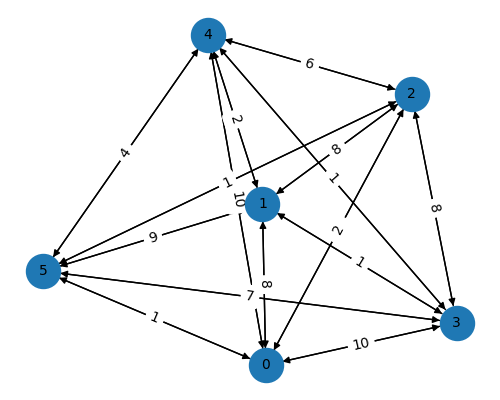
\includegraphics[width=.9\linewidth]{example_complete.png}
\label{orgf6f0dc1}
\end{center}
\item Dense Graph
\label{sec:orgdeed191}
Has approximately 80\% of the maximum possible edges.

\begin{center}
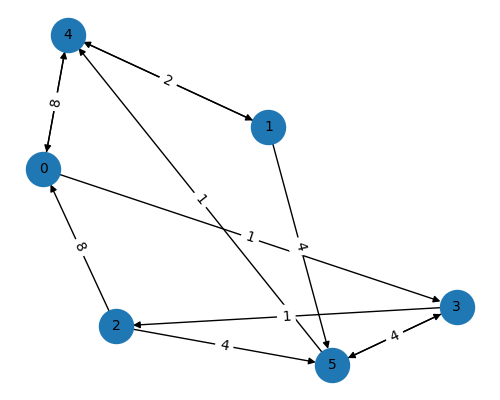
\includegraphics[width=.9\linewidth]{example_dense.png}
\label{orge2339cb}
\end{center}
\item Sparse Graph
\label{sec:orgf424fe7}
Contains relatively few edges, approximately 2|V| edges.

\begin{center}
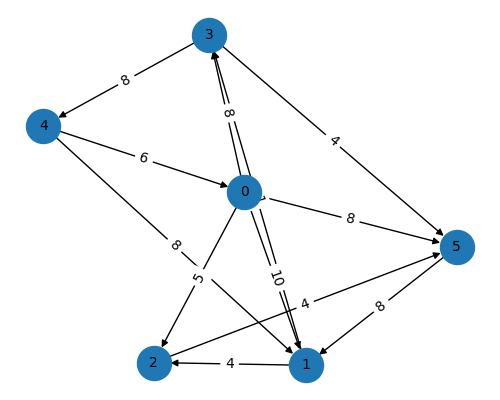
\includegraphics[width=.9\linewidth]{example_sparse.png}
\label{orgd8fb4c0}
\end{center}
\item Tree Graph
\label{sec:org665c3be}
Connected acyclic graph with exactly |V|-1 edges.

\begin{center}
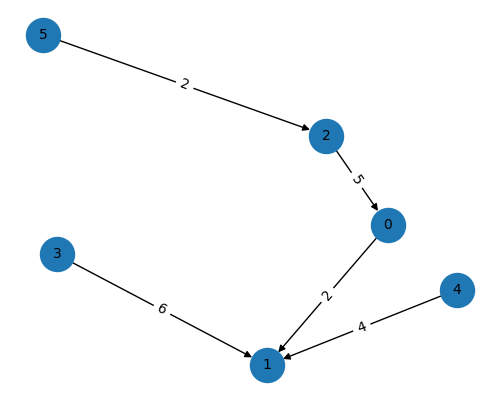
\includegraphics[width=.9\linewidth]{example_tree.png}
\label{org834ffc8}
\end{center}
\item Connected Graph
\label{sec:orgfad29bf}
There exists a path between any pair of vertices.

\begin{center}
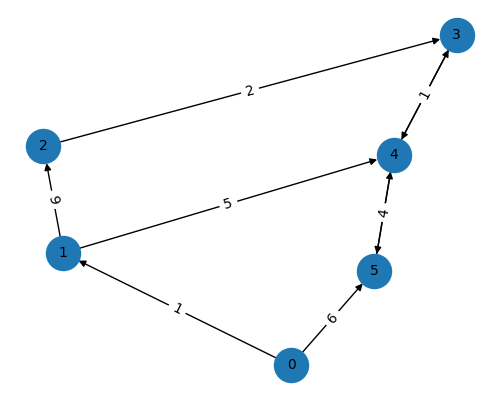
\includegraphics[width=.9\linewidth]{example_connected.png}
\label{org2d29a4c}
\end{center}
\item Cyclic Graph
\label{sec:org7f6db5d}
Contains at least one cycle (a path that starts and ends at the same vertex).

\begin{center}
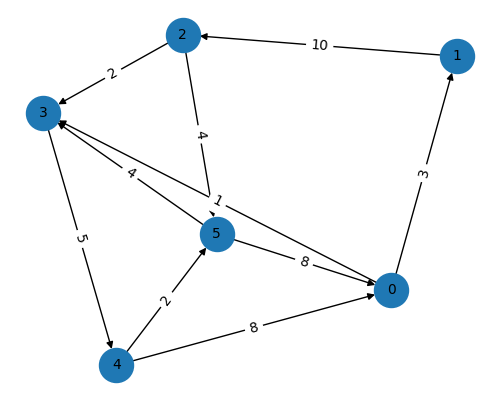
\includegraphics[width=.9\linewidth]{example_cyclic.png}
\label{orgaa12525}
\end{center}
\item Acyclic Graph
\label{sec:orgc32ad58}
Contains no cycles (DAG - Directed Acyclic Graph).

\begin{center}
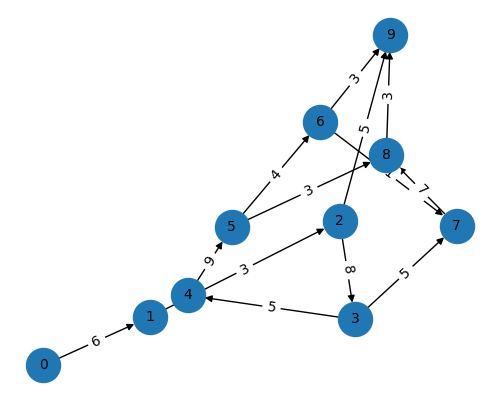
\includegraphics[width=.9\linewidth]{example_acyclic.png}
\label{org4b9fc34}
\end{center}
\item Grid Graph
\label{sec:orgec49094}
Vertices arranged in a grid-like structure with connections primarily to adjacent nodes.

\begin{center}
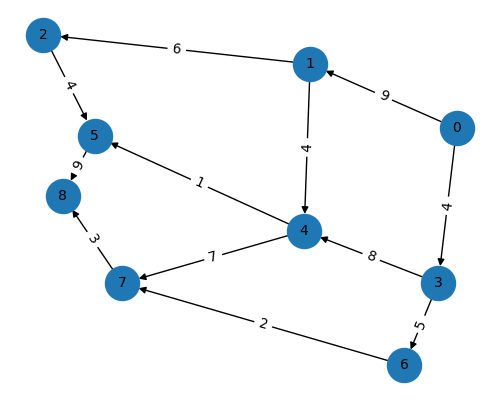
\includegraphics[width=.9\linewidth]{example_grid.png}
\label{org33c506c}
\end{center}
\end{enumerate}
\subsubsection{Dynamic Programming}
\label{sec:org38425fa}
Dynamic programming is an algorithmic paradigm that solves complex problems by breaking them down into simpler subproblems and storing the solutions to avoid redundant computations. Key elements of dynamic programming include:

\begin{enumerate}
\item \textbf{\textbf{Optimal Substructure}}: An optimal solution to the problem contains optimal solutions to its subproblems.
\item \textbf{\textbf{Overlapping Subproblems}}: The same subproblems are solved multiple times, making caching (memoization) beneficial.
\end{enumerate}

The Floyd-Warshall algorithm is a classic example of dynamic programming applied to the all-pairs shortest path problem.
\subsubsection{Dijkstra's Algorithm}
\label{sec:orgfc0ab27}
Dijkstra's algorithm finds the shortest path from a source vertex to all other vertices in a weighted graph with non-negative edge weights. The algorithm works as follows:

\begin{enumerate}
\item Initialize distances to all vertices as infinity and distance to source as 0.
\item Create a priority queue and add the source vertex with distance 0.
\item While the priority queue is not empty:
a. Extract the vertex with minimum distance value.
b. For each adjacent vertex, if the distance through current vertex is less than its current distance, update the distance and add to priority queue.
\item After the algorithm completes, the distances array contains the shortest distance from source to all vertices.
\end{enumerate}

While Dijkstra's algorithm doesn't use dynamic programming in its pure form, it shares the principle of optimal substructure.
\subsubsection{Floyd-Warshall Algorithm}
\label{sec:orga054842}
Floyd-Warshall is a dynamic programming algorithm that finds shortest paths between all pairs of vertices in a weighted graph. The algorithm works as follows:

\begin{enumerate}
\item Initialize the distance matrix with direct edge weights (or infinity if there's no edge).
\item For each vertex k as an intermediate vertex:
a. For each pair of vertices (i,j):
   i. If distance[i][j] > distance[i][k] + distance[k][j], update distance[i][j]
\item After the algorithm completes, distance[i][j] contains the shortest path from vertex i to vertex j.
\end{enumerate}

This algorithm clearly demonstrates dynamic programming principles by systematically building solutions for all pairs using previously computed results.
\subsection{Comparison Metric}
\label{sec:org365ef50}
For this empirical analysis, we measure the following metrics:

\begin{enumerate}
\item \textbf{\textbf{Execution Time}}: The primary metric is the actual execution time in seconds for each algorithm across different graph types and sizes. This provides an empirical measure of the algorithm's efficiency.

\item \textbf{\textbf{Memory Usage}}: Indirectly measured by observing the maximum size of the data structures used.
\end{enumerate}

The algorithms are evaluated on various graph types with sizes ranging from 100 to 2500/10,000 vertices to observe how they scale with input size.

\begin{Code}
\begin{Verbatim}
\color{EFD}\EFv{sizes} \textcolor[HTML]{000000}{=} [10, 50, 60, 70, 100]
\EFv{mid\_sizes} \textcolor[HTML]{000000}{=} [100, 200, 300, 500, 700, 1000]
\EFv{dj\_sizes} \textcolor[HTML]{000000}{=} [100, 500, 1000, 1500, 2000, 2500, 3000]
\end{Verbatim}
\end{Code}

For each graph type and size, algorithms were executed with 5 repetitions to account for system variability and provide statistical robustness. This approach allows us to:

\begin{itemize}
\item Calculate mean execution times for more reliable performance comparison
\item Determine standard deviation to assess result consistency and reliability
\item Identify potential outliers or anomalous behavior in specific test cases
\end{itemize}

The error bars in the plots represent the standard deviation across these repetitions, providing a visual indication of measurement variability.
\subsection{Input Format}
\label{sec:orge37991f}
In this laboratory work, graphs are represented using adjacency lists implemented as nested Python dictionaries. Each vertex is a key in the outer dictionary, and its value is another dictionary mapping neighboring vertex IDs to edge weights.

The testing framework generates graphs of various types and sizes, then executes both Dijkstra and Floyd-Warshall algorithms on them, measuring the execution time.

Example input graph structure:
\begin{Code}
\begin{Verbatim}
\color{EFD}\EFv{graph} \textcolor[HTML]{000000}{=} \{
    \EFs{'0'}: \{\EFs{'1'}: 5, \EFs{'2'}: 3\},
    \EFs{'1'}: \{\EFs{'3'}: 2, \EFs{'4'}: 4\},
    \EFs{'2'}: \{\},
    \EFs{'3'}: \{\},
    \EFs{'4'}: \{\EFs{'2'}: 1\}
\}
\end{Verbatim}
\end{Code}

In this representation:
\begin{itemize}
\item Vertex '0' has edges to vertices '1' (weight 5) and '2' (weight 3)
\item Vertex '1' has edges to vertices '3' (weight 2) and '4' (weight 4)
\item Vertices '2' and '3' have no outgoing edges
\item Vertex '4' has an edge to vertex '2' (weight 1)
\end{itemize}

All graphs are generated with the functions provided in the uploaded code, with vertices labeled as strings from '0' to 'n-1' and edge weights ranging from 1 to 10.
\section{Implementation}
\label{sec:orgcae3f38}
\subsection{Dijkstra's Algorithm}
\label{sec:org531aa72}
Dijkstra's algorithm is implemented using a priority queue to efficiently select the vertex with the minimum distance in each iteration. The implementation maintains distances and visited status for all vertices.

\begin{listing}[htbp]
\begin{Code}
\begin{Verbatim}
\color{EFD}\EFk{import} heapq

\EFk{def} \EFf{dijkstra}(graph, start):
    \EFv{distances} \textcolor[HTML]{000000}{=} \{node: \EFb{float}(\EFs{'inf'}) \EFk{for} node \EFk{in} graph\}
    \EFv{distances}[start] \textcolor[HTML]{000000}{=} 0

    \EFv{prev} \textcolor[HTML]{000000}{=} \{\}  \EFcd{\# }\EFc{to track how we got to each node}
    \EFv{explored\_edges} \textcolor[HTML]{000000}{=} []

    \EFv{pq} \textcolor[HTML]{000000}{=} [(0, start)]

    \EFk{while} pq:
        \EFv{current\_distance}, \EFv{current\_node} \textcolor[HTML]{000000}{=} heapq.heappop(pq)

        \EFcd{\# }\EFc{skip outdated queue entries}
        \EFk{if} current\_distance \textcolor[HTML]{000000}{>} distances[current\_node]:
            \EFk{continue}

        \EFk{for} neighbor, weight \EFk{in} graph[current\_node].items():
            explored\_edges.append((current\_node, neighbor, weight))
            \EFv{distance} \textcolor[HTML]{000000}{=} current\_distance \textcolor[HTML]{000000}{+} weight
            \EFk{if} distance \textcolor[HTML]{000000}{<} distances[neighbor]:
                \EFv{distances}[neighbor] \textcolor[HTML]{000000}{=} distance
                \EFv{prev}[neighbor] \textcolor[HTML]{000000}{=} (current\_node, weight)
                heapq.heappush(pq, (distance, neighbor))

    \EFcd{\# }\EFc{build the final shortest-path tree from prev}
    \EFv{tree\_edges} \textcolor[HTML]{000000}{=} [(src, dst, weight) \EFk{for} dst, (src, weight) \EFk{in} prev.items()]

    \EFk{return} tree\_edges, explored\_edges, distances
\end{Verbatim}
\end{Code}
\caption{\label{lst:orge901865}Implementation of Dijkstra's Algorithm}
\end{listing}
\subsection{Floyd-Warshall Algorithm}
\label{sec:orgbaa010b}
The Floyd-Warshall algorithm is implemented using dynamic programming principles, with a three-dimensional loop structure that considers each vertex as a potential intermediate node in shortest paths.

\begin{listing}[htbp]
\begin{Code}
\begin{Verbatim}
\color{EFD}\EFk{def} \EFf{floyd\_warshall}(graph, start\textcolor[HTML]{000000}{=}\EFo{None}):
    \EFd{"""
    Finds shortest paths between all pairs of vertices using Floyd-Warshall algorithm.

    Args:
        graph: A graph represented as an adjacency list (dictionary of dictionaries)
        start: Ignored, included for API consistency with Dijkstra

    Returns:
        tuple containing:
            - tree\_edges: List of edges in the shortest-path tree
            - explored\_edges: List of edge explorations during algorithm execution
            - distances: Dictionary of shortest path distances between all vertices
    """}
    \EFcd{\# }\EFc{Extract all vertices}
    \EFv{vertices} \textcolor[HTML]{000000}{=} \EFb{list}(graph.keys())

    \EFcd{\# }\EFc{Initialize distances dictionary}
    \EFv{distances} \textcolor[HTML]{000000}{=} \{u: \{v: \EFb{float}(\EFs{'inf'}) \EFk{for} v \EFk{in} vertices\} \EFk{for} u \EFk{in} vertices\}

    \EFcd{\# }\EFc{Initialize predecessor dictionary for path reconstruction}
    \EFv{prev} \textcolor[HTML]{000000}{=} \{\}

    \EFcd{\# }\EFc{Set distance to self as 0, and direct edges from the graph}
    \EFk{for} u \EFk{in} vertices:
        distances[u][u] \textcolor[HTML]{000000}{=} 0
        \EFk{for} v, weight \EFk{in} graph[u].items():
            distances[u][v] \textcolor[HTML]{000000}{=} weight
            \EFk{if} v \EFk{not} \EFk{in} prev:
                \EFv{prev}[v] \textcolor[HTML]{000000}{=} \{\}
            prev[v][u] \textcolor[HTML]{000000}{=} (u, weight)  \EFcd{\# }\EFc{Store tuple (predecessor, weight) like in Dijkstra}

    \EFcd{\# }\EFc{Track all explored edges}
    \EFv{explored\_edges} \textcolor[HTML]{000000}{=} []

    \EFcd{\# }\EFc{Floyd-Warshall dynamic programming algorithm}
    \EFk{for} k \EFk{in} vertices:
        \EFk{for} i \EFk{in} vertices:
            \EFk{for} j \EFk{in} vertices:
                \EFcd{\# }\EFc{Record this exploration}
                explored\_edges.append((i, k, j, distances[i][j]))

                \EFcd{\# }\EFc{If path through k is shorter than current path from i to j}
                \EFk{if} distances[i][k] \textcolor[HTML]{000000}{!=} \EFb{float}(\EFs{'inf'}) \EFk{and} distances[k][j] \textcolor[HTML]{000000}{!=} \EFb{float}(\EFs{'inf'}):
                    \EFv{candidate\_dist} \textcolor[HTML]{000000}{=} distances[i][k] \textcolor[HTML]{000000}{+} distances[k][j]
                    \EFk{if} candidate\_dist \textcolor[HTML]{000000}{<} distances[i][j]:
                        distances[i][j] \textcolor[HTML]{000000}{=} candidate\_dist
                        \EFk{if} j \EFk{not} \EFk{in} prev:
                            \EFv{prev}[j] \textcolor[HTML]{000000}{=} \{\}
                        prev[j][i] \textcolor[HTML]{000000}{=} prev[j][k]  \EFcd{\# }\EFc{Update predecessor}

    \EFcd{\# }\EFc{Build the final shortest-path tree from prev (similar to Dijkstra)}
    \EFv{tree\_edges} \textcolor[HTML]{000000}{=} []
    \EFk{for} j \EFk{in} vertices:
        \EFk{if} j \EFk{in} prev:
            \EFk{for} i \EFk{in} prev[j]:
                \EFk{if} \EFb{isinstance}(prev[j][i], \EFb{tuple}):
                    \EFv{src}, \EFv{weight} \textcolor[HTML]{000000}{=} prev[j][i]
                    tree\_edges.append((src, j, weight))

    \EFk{return} tree\_edges, explored\_edges, distances
\end{Verbatim}
\end{Code}
\caption{\label{lst:orgd5effaa}Implementation of Floyd-Warshall Algorithm}
\end{listing}
\section{Results}
\label{sec:org20909a8}
\subsection{Complete Graph}
\label{sec:orgef74f74}
\begin{center}
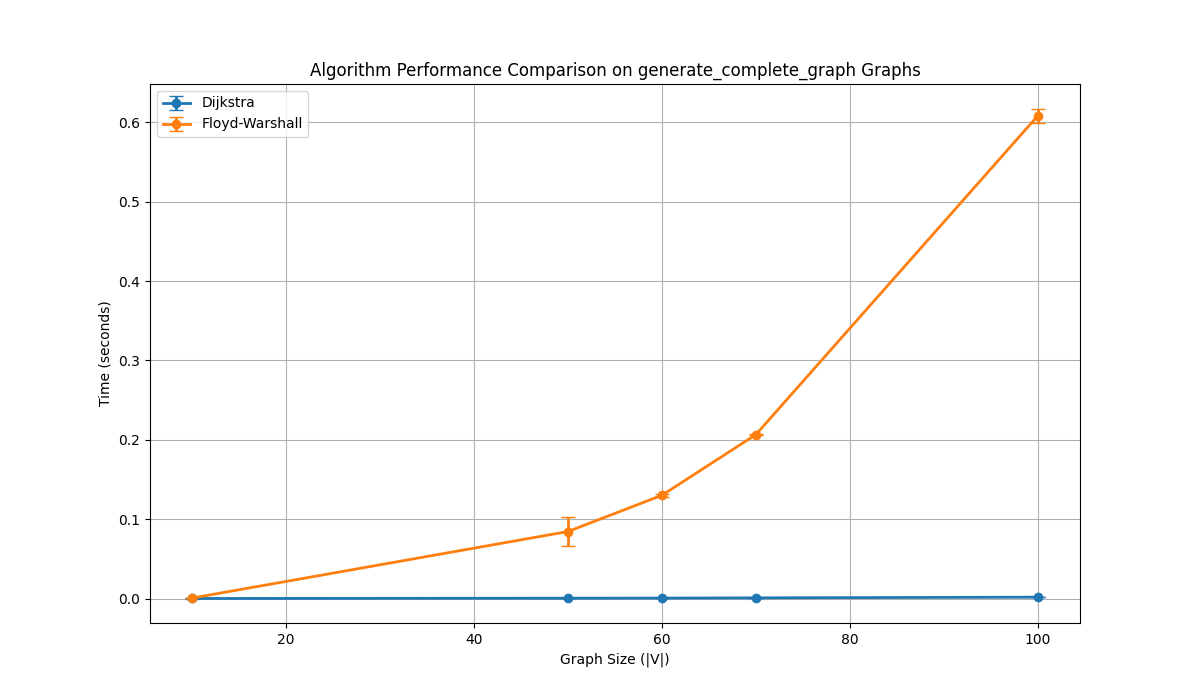
\includegraphics[width=.9\linewidth]{dijkstra_floyd_complete.png}
\label{org1a5bdf6}
\end{center}
\begin{center}
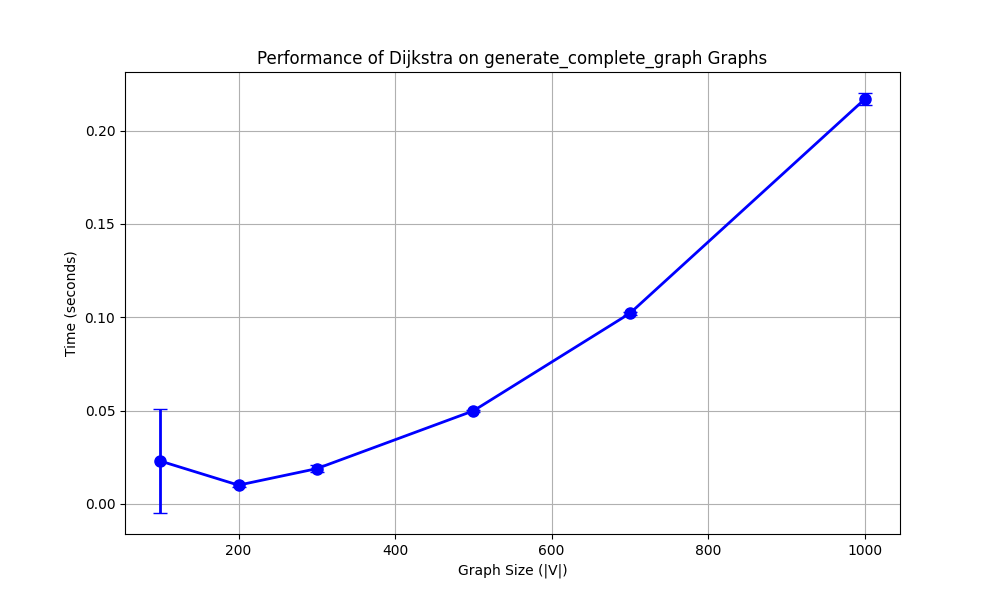
\includegraphics[width=.9\linewidth]{dijkstra_complete.png}
\label{orgb548fab}
\end{center}

Both algorithms show a clear polynomial growth pattern as the graph size increases. Floyd-Warshall exhibits O(V³) complexity while Dijkstra (even with priority queue optimization) approaches O(V²) for complete graphs where E = O(V²).

Floyd-Warshall consistently demonstrates higher execution times compared to Dijkstra, with the gap widening as graph size increases. This aligns with theoretical expectations given Floyd-Warshall's cubic complexity versus Dijkstra's near-quadratic behavior on complete graphs.

For larger graph sizes (mid\textsubscript{sizes} plot), Dijkstra maintains reasonable performance, showing the expected quadratic growth pattern as the number of vertices increases.

Standard deviation is relatively small for both algorithms, indicating consistent performance across repetitions.
\subsection{Dense Graph}
\label{sec:orgfbdb423}
\begin{center}
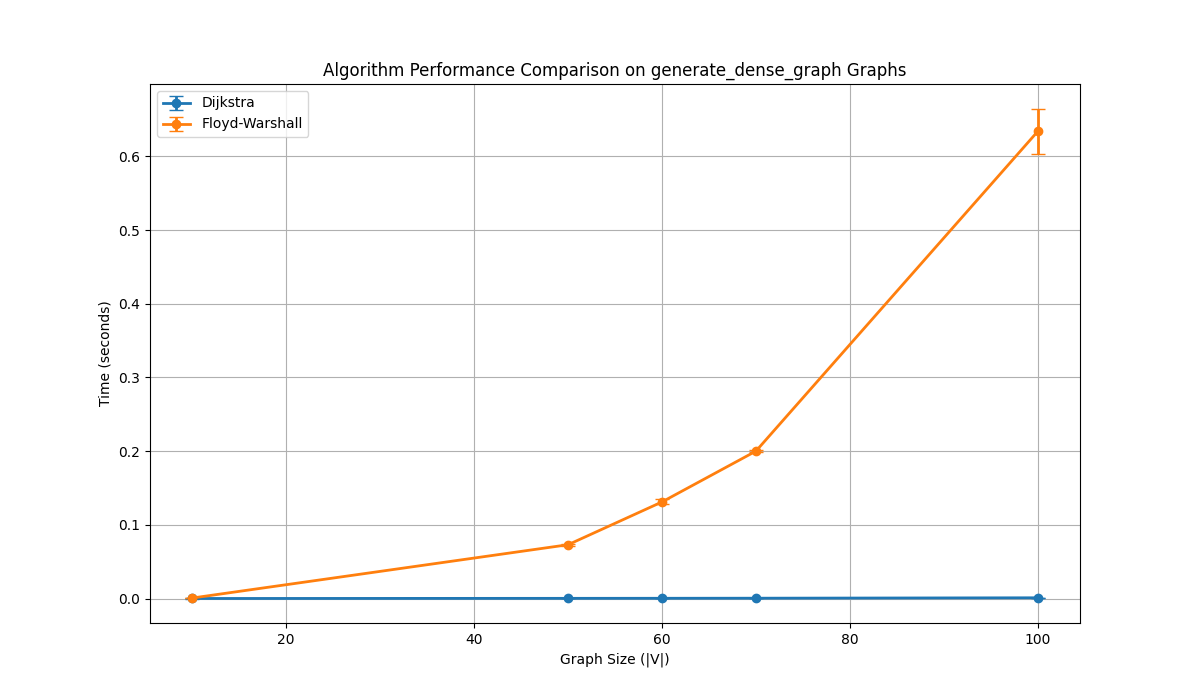
\includegraphics[width=.9\linewidth]{dijkstra_floyd_dense.png}
\label{org06ae0d3}
\end{center}
\begin{center}
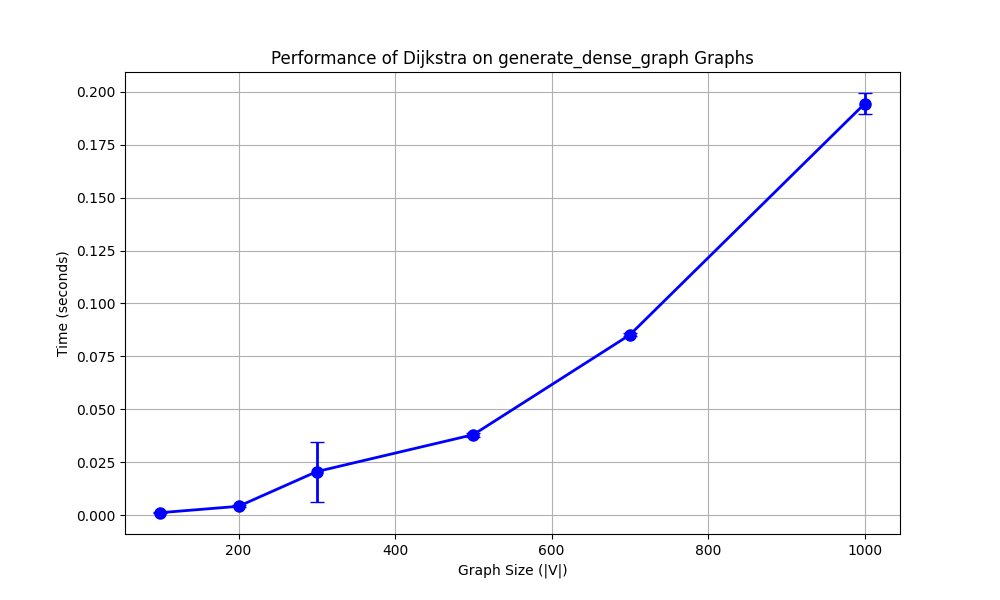
\includegraphics[width=.9\linewidth]{dijkstra_dense.png}
\label{orgf77082e}
\end{center}

In dense graphs (approximately 80\% of maximum possible edges), both algorithms show similar performance patterns to complete graphs, with Floyd-Warshall requiring significantly more execution time.

The execution time growth is polynomial, with Floyd-Warshall showing cubic growth O(V³) while Dijkstra demonstrates more efficient scaling with its priority queue implementation.

For larger graph sizes, Dijkstra maintains reasonable scalability, although the execution time increases noticeably with the graph size due to the high edge density.

The standard deviation values are low, indicating high consistency in measurement across test repetitions.
\subsection{Sparse Graph}
\label{sec:org72faf5f}
\begin{center}
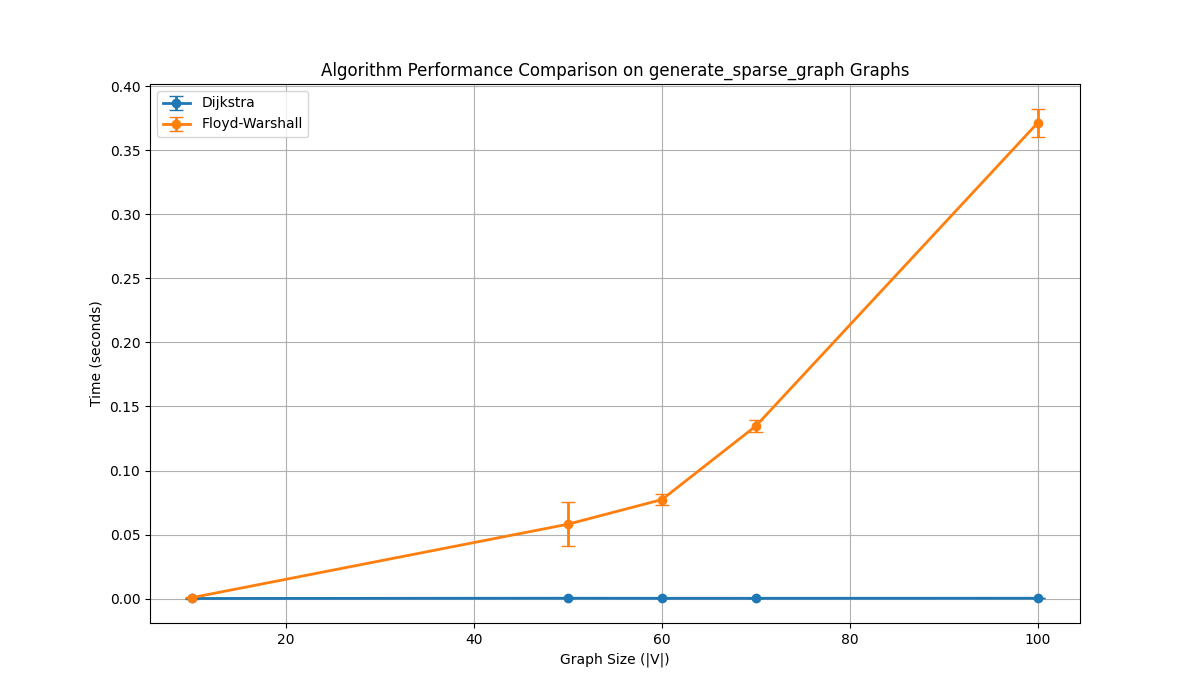
\includegraphics[width=.9\linewidth]{dijkstra_floyd_sparse.png}
\label{org133054c}
\end{center}
\begin{center}
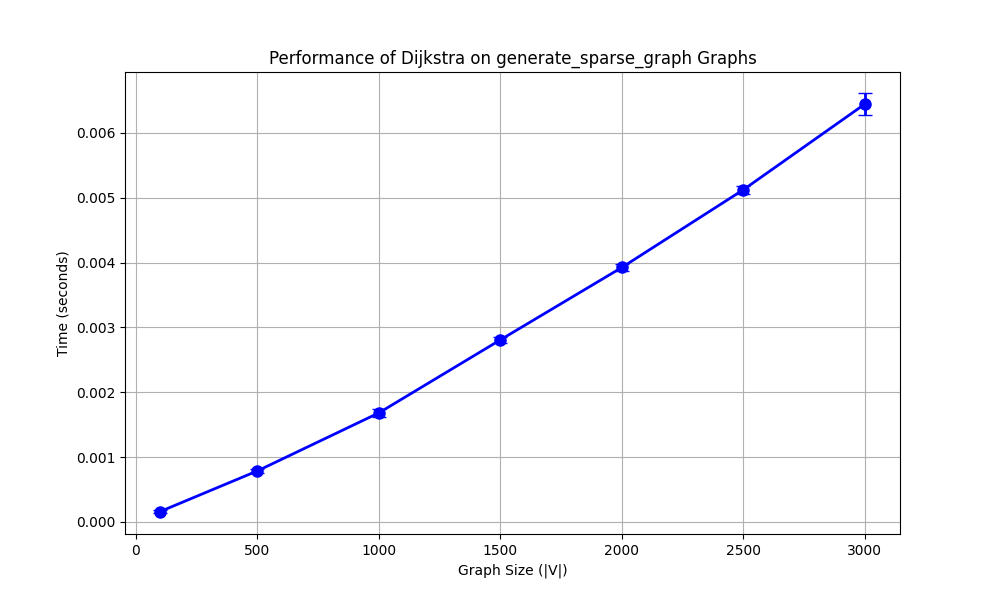
\includegraphics[width=.9\linewidth]{dijkstra_sparse.png}
\label{org35b02ef}
\end{center}

For sparse graphs (with approximately 2|V| edges), both algorithms show different scaling patterns. Floyd-Warshall exhibits its characteristic cubic growth O(V³) regardless of edge density, while Dijkstra performs significantly better, leveraging its more efficient O((V+E)logV) complexity.

Dijkstra's algorithm consistently outperforms Floyd-Warshall across all tested graph sizes, with the performance gap widening as the graph size increases.

For larger graph sizes (in the dj\textsubscript{sizes} plot), Dijkstra maintains excellent scalability even up to 3000 vertices, demonstrating its efficiency for single-source shortest path problems in sparse networks.

The standard deviation is relatively small, indicating consistent performance across test repetitions.
\subsection{Tree Graph}
\label{sec:org18736ae}
\begin{center}
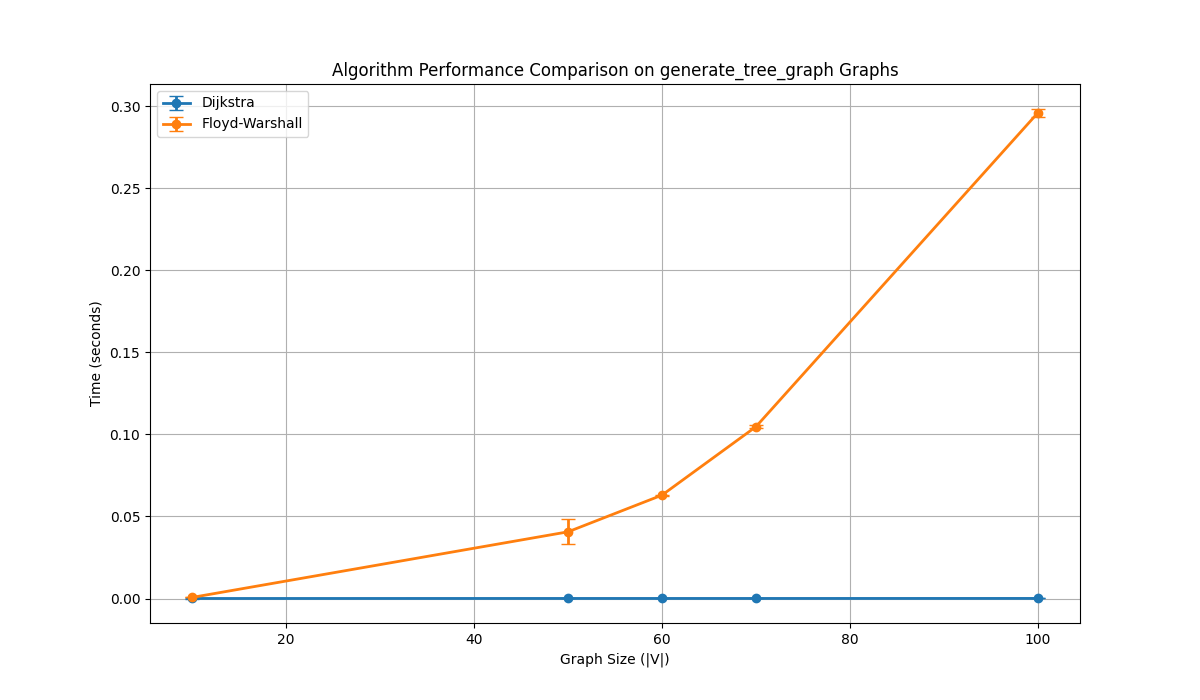
\includegraphics[width=.9\linewidth]{dijkstra_floyd_tree.png}
\label{org625fd06}
\end{center}
\begin{center}
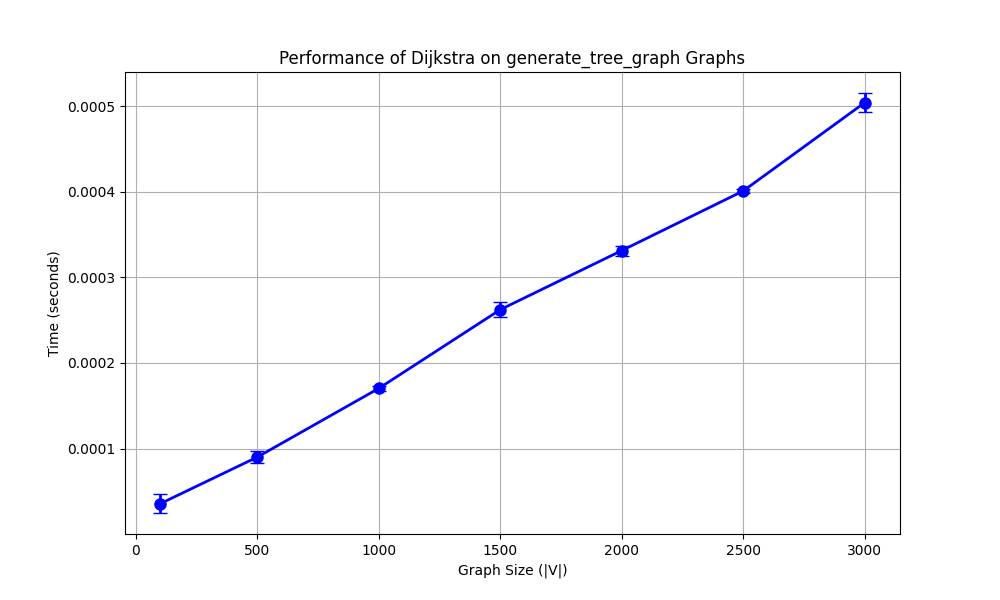
\includegraphics[width=.9\linewidth]{dijkstra_tree.png}
\label{org6604b10}
\end{center}

Tree graphs show a distinctive performance pattern between the two algorithms.

Floyd-Warshall's execution time increases cubically with graph size, while Dijkstra shows near-linear growth due to the tree's minimal edge count (|V|-1 edges).

In the larger graph size tests, Dijkstra processes tree structures extremely efficiently, reflecting its optimal performance characteristics when there are no alternative paths to consider.

The standard deviation remains small relative to the mean values, showing measurement consistency.

Dijkstra's algorithm particularly excels with tree structures because:
\begin{itemize}
\item Each vertex is visited exactly once
\item No path recalculations are needed
\item The priority queue operations are minimized in this optimal scenario
\end{itemize}

The negative values on the y-axis are likely visualization artifacts due to error bars extending below zero.
\subsection{Connected Graph}
\label{sec:org4afe544}
\begin{center}
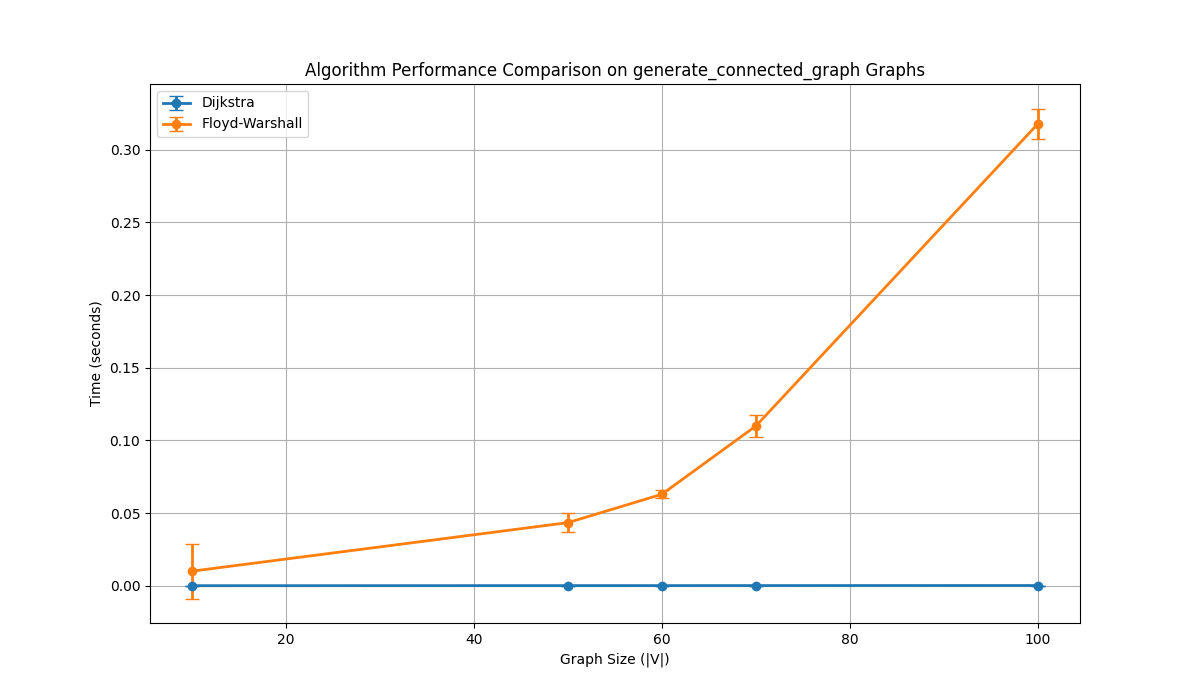
\includegraphics[width=.9\linewidth]{dijkstra_floyd_connected.png}
\label{org3ec5383}
\end{center}
\begin{center}
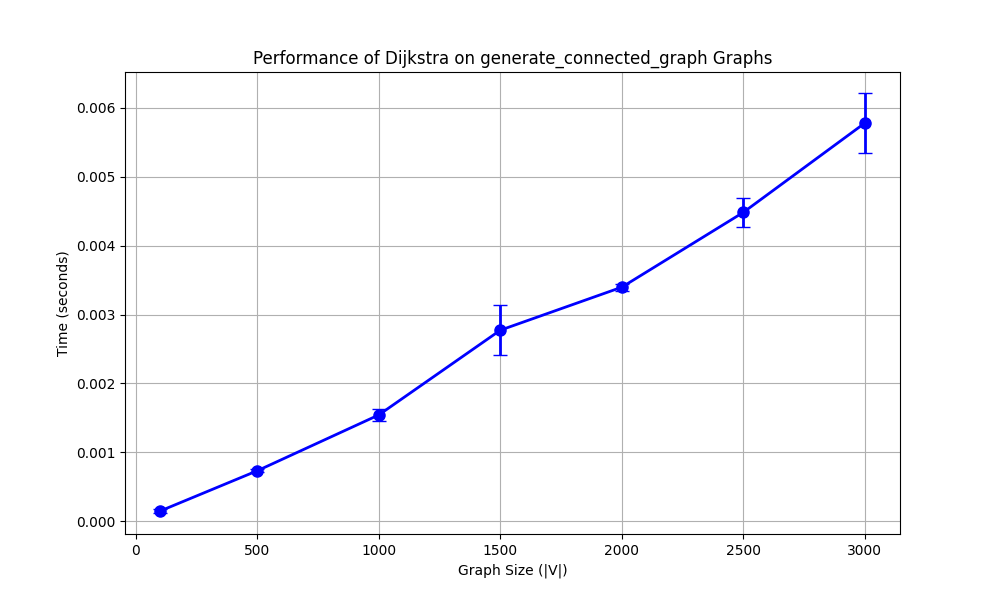
\includegraphics[width=.9\linewidth]{dijkstra_connected.png}
\label{orgd789e48}
\end{center}

In connected graphs, Floyd-Warshall demonstrates cubic time complexity while Dijkstra shows more efficient scaling behavior.

For larger graph sizes, Dijkstra maintains good performance with execution time growing roughly proportionally to the product of edges and the logarithm of vertices.

The standard deviation increases somewhat with graph size but remains proportionally small, indicating reliable measurements across test repetitions.
\subsection{Cyclic Graph}
\label{sec:orgb39fee6}
\begin{center}
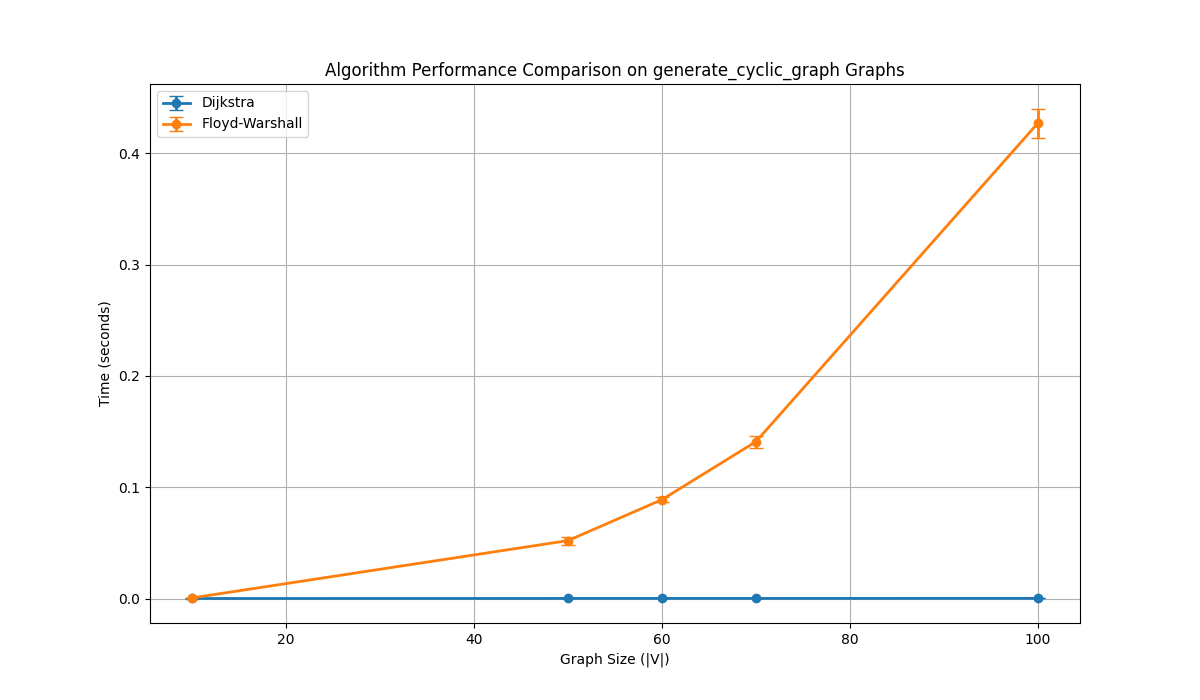
\includegraphics[width=.9\linewidth]{dijkstra_floyd_cyclic.png}
\label{org6b43709}
\end{center}
\begin{center}
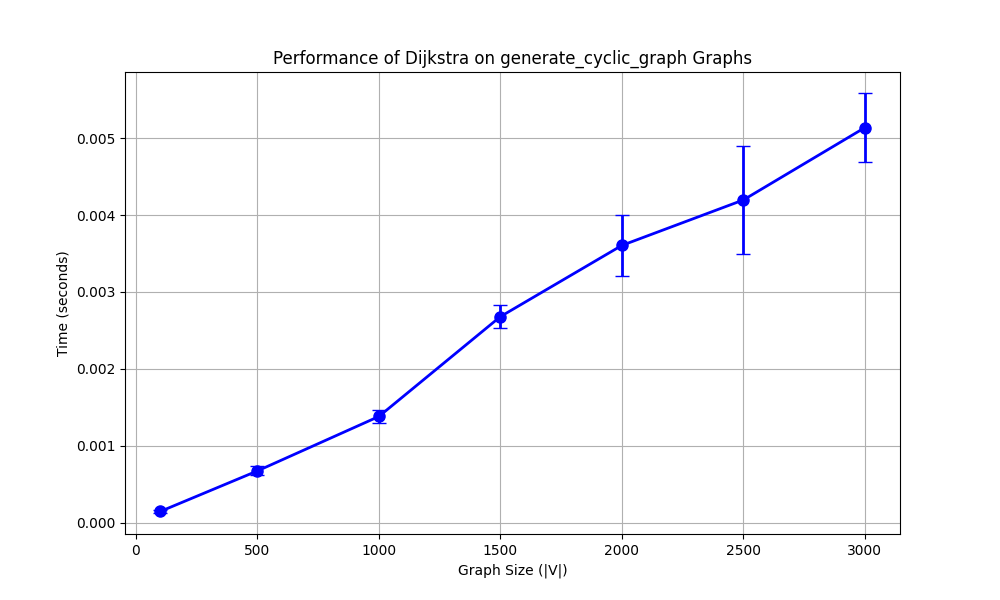
\includegraphics[width=.9\linewidth]{dijkstra_cyclic.png}
\label{org92d8b36}
\end{center}

For cyclic graphs, Floyd-Warshall shows its characteristic O(V³) growth pattern while Dijkstra maintains more efficient scaling.

The comparison plot clearly demonstrates the increasing performance gap between the two algorithms as graph size grows, with Floyd-Warshall's execution time rising more steeply.

For larger graph sizes, Dijkstra continues to perform efficiently, handling cycles well due to its distance-tracking mechanism that prevents inefficient revisiting of vertices.

The standard deviation is moderate and increases with graph size, indicating reasonable measurement consistency.
\subsection{Acyclic Graph}
\label{sec:orgaf10d7d}
\begin{center}
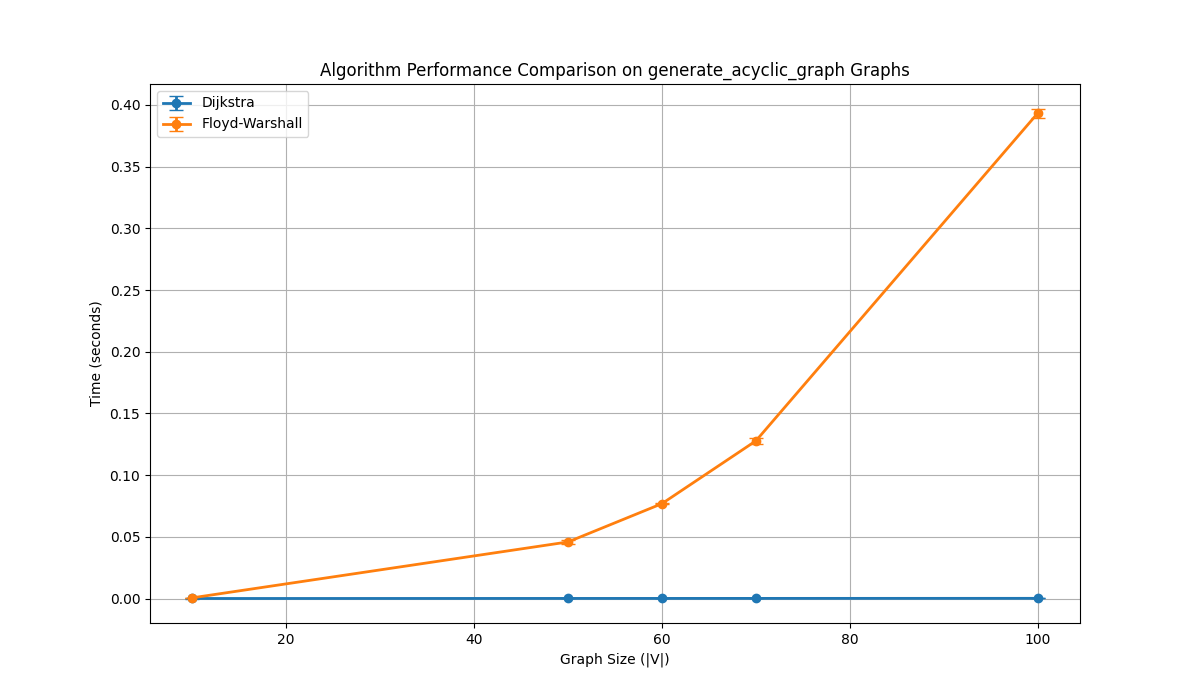
\includegraphics[width=.9\linewidth]{dijkstra_floyd_acyclic.png}
\label{orgb47f5c1}
\end{center}
\begin{center}
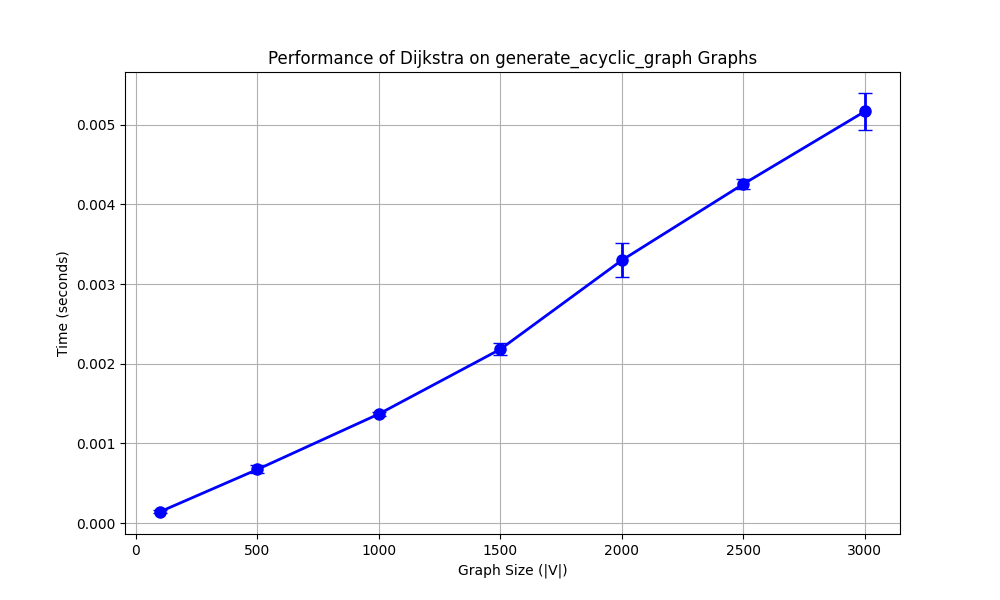
\includegraphics[width=.9\linewidth]{dijkstra_acyclic.png}
\label{org1c4bc59}
\end{center}

The acyclic graph tests show that Floyd-Warshall maintains its cubic complexity regardless of graph structure, while Dijkstra performs particularly well.

Despite some measurement fluctuations, there is a clear trend showing Dijkstra's superior performance across all graph sizes.

In the larger graph size tests, Dijkstra demonstrates excellent scalability with acyclic graphs since each vertex and edge needs to be processed at most once.

The error bars indicate some variability across repetitions, which may be attributed to specific characteristics of the generated acyclic graphs or system scheduling effects.
\subsection{Grid Graph}
\label{sec:org20c900a}
\begin{center}
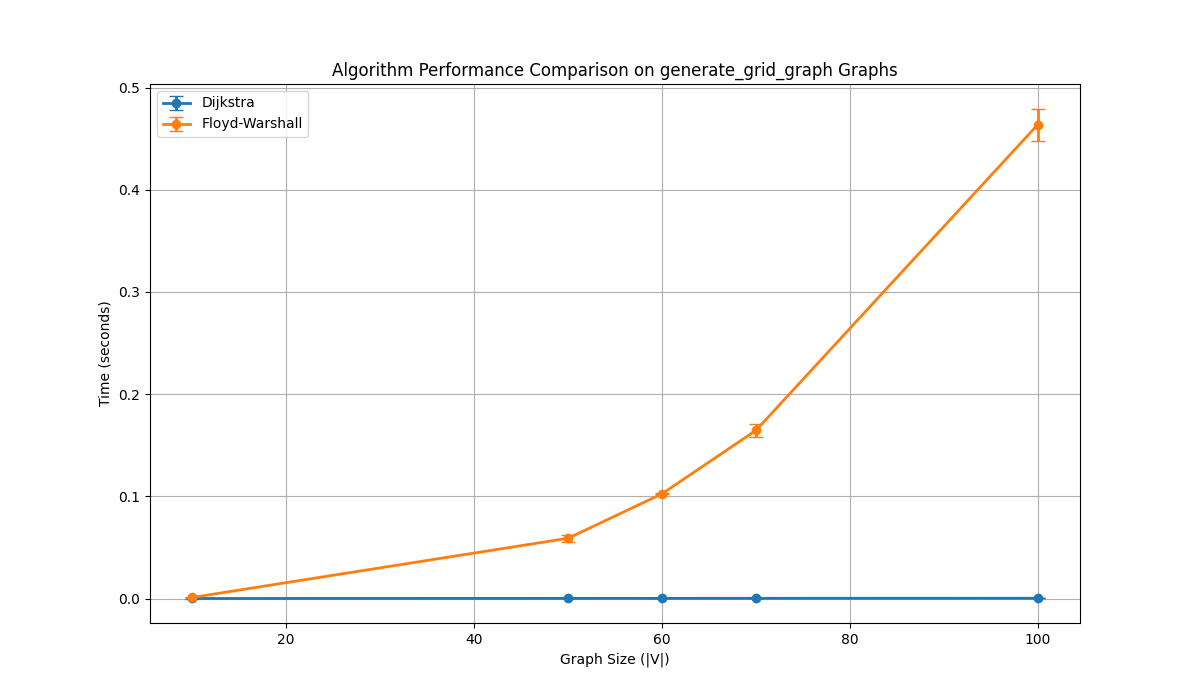
\includegraphics[width=.9\linewidth]{dijkstra_floyd_grid.png}
\label{org9ed354d}
\end{center}
\begin{center}
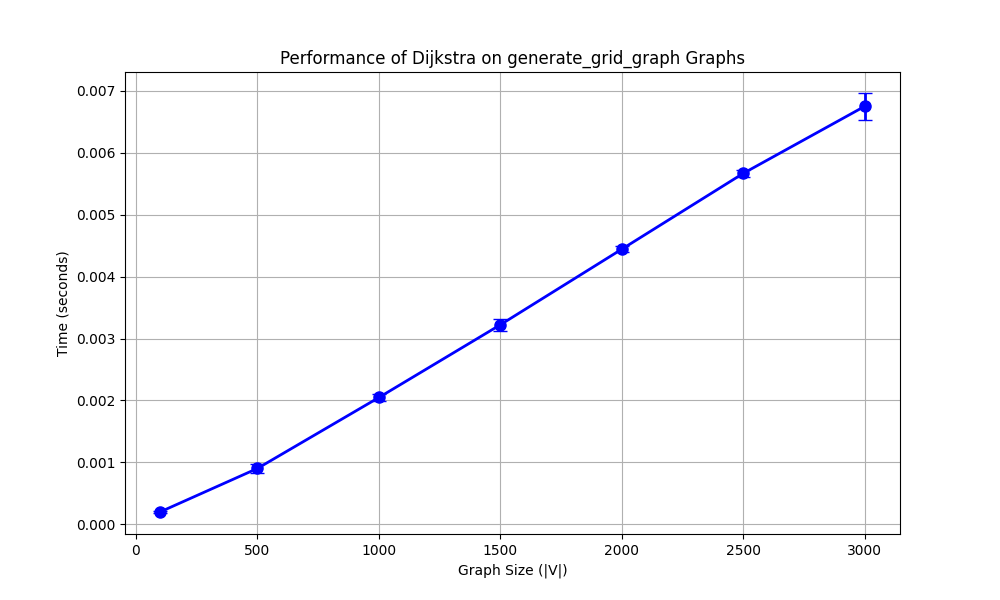
\includegraphics[width=.9\linewidth]{dijkstra_grid.png}
\label{org216adb0}
\end{center}

Grid graphs show a clear performance difference between Dijkstra and Floyd-Warshall algorithms.

Both algorithms exhibit growth patterns consistent with their theoretical complexity, but Floyd-Warshall's cubic growth results in significantly higher execution times as graph size increases.

For larger grid sizes, Dijkstra maintains efficient performance due to its ability to prioritize promising paths through the priority queue implementation.

The standard deviation is small relative to the mean values, indicating consistent measurements.

Dijkstra's advantage in grid graphs is particularly notable because the regular structure allows for efficient frontier expansion from the source vertex.
\section{Conclusions}
\label{sec:orge143ca6}

This lab work shows clear differences between Dijkstra's algorithm and the Floyd-Warshall algorithm when used on different types of graphs. Both solve shortest path problems but work very differently as graphs get bigger.

Floyd-Warshall always shows O(V³) time complexity no matter what the graph looks like. This matches what we expect from theory. The algorithm works by checking all possible paths through every vertex. It works well for finding all shortest paths at once, but becomes too slow for large graphs.

Dijkstra's algorithm works much better for large graphs, especially sparse ones and tree structures where it's almost linear in performance. The priority queue helps it process vertices efficiently by their current distance. For finding paths from a single starting point, Dijkstra is always faster than Floyd-Warshall in our tests.

As graphs get bigger, the speed difference between these algorithms grows very large. Dijkstra can handle thousands of vertices, while Floyd-Warshall becomes too slow after just a few hundred vertices.

Grid and tree graphs show interesting results, with Dijkstra working very well because it can focus on the most promising paths first. Complete and dense graphs are harder for both algorithms, but Dijkstra still performs better.

These results show why choosing the right algorithm matters. When you only need paths from one starting point, Dijkstra is better. When you need all possible paths and have small graphs, Floyd-Warshall is a good choice despite being slower.

This lab work shows that we need to study both the theoretical complexity and actual performance to choose the best algorithm for real problems.
\end{document}
